\section{Simulation of the Shunt Active Filter Operating with an Electrohidraulic Actuator}

The operation of the shunt active filter in an aircraft electrical system was evaluated by simulation. The system is composed of the generation and distribution system and some loads constituted by electrohydraulic actuators (EHAs) with shunt active filters connected to its respective inputs.

\subsection{Active Filter Model}

The shunt active filter consists of a Current Reference Calculator and a Compensator, as shown in Fig. \ref{fig:filtro_blocos_1.png}. This figure shows these parts with its respective internal sub-blocks. The Current Reference Calculator block is comprised by the Positive Sequence Detector (Fig. \ref{fig:detector_seq_positiva.png}) and the Active Filter Reference Definition (Fig. \ref{fig:diagrama_filtro.png}). These sub-blocks are responsible for the calculation algorithm (each sub-block presents its respective signals inputs and outputs) to determine the reference to be applied in the compensator. The Compensator is presented by the VSC with its respective hysteresis controller and capacitor voltage PI controller. This figure shows also the voltages and currents measurement probes connection in the electrical grid, where acquire the inputs for the active filter operation.

The reference calculator block defines the proper reference to be applied in the compensator. Its inputs are the load currents and the grid voltages measurements, while its output is the reference applied to the compensator. The compensator block consists of a VSC with its capacitor DC voltage regulated by a closed-loop controller. The compensator also has the hysteresis controller, which creates the commands applied to the VSC switching devices.

The shunt active filter operation requires a passive capacitor filter applied in the transmission lines to eliminate the high frequency content injected in the system by the switching commutation \citep{Akagi2007}. Due to high switching commutation frequency, the passive filter is lightweight and does not impact significantly in the aircraft system. However, the presence of capacitors in the transmission lines may decrease the power factor due to the voltage and current phase angle shift. To eliminate this, inductors may be applied in the lines to compensate the reactive power flow.

\begin{figure*}[!tb] %
	\centering
	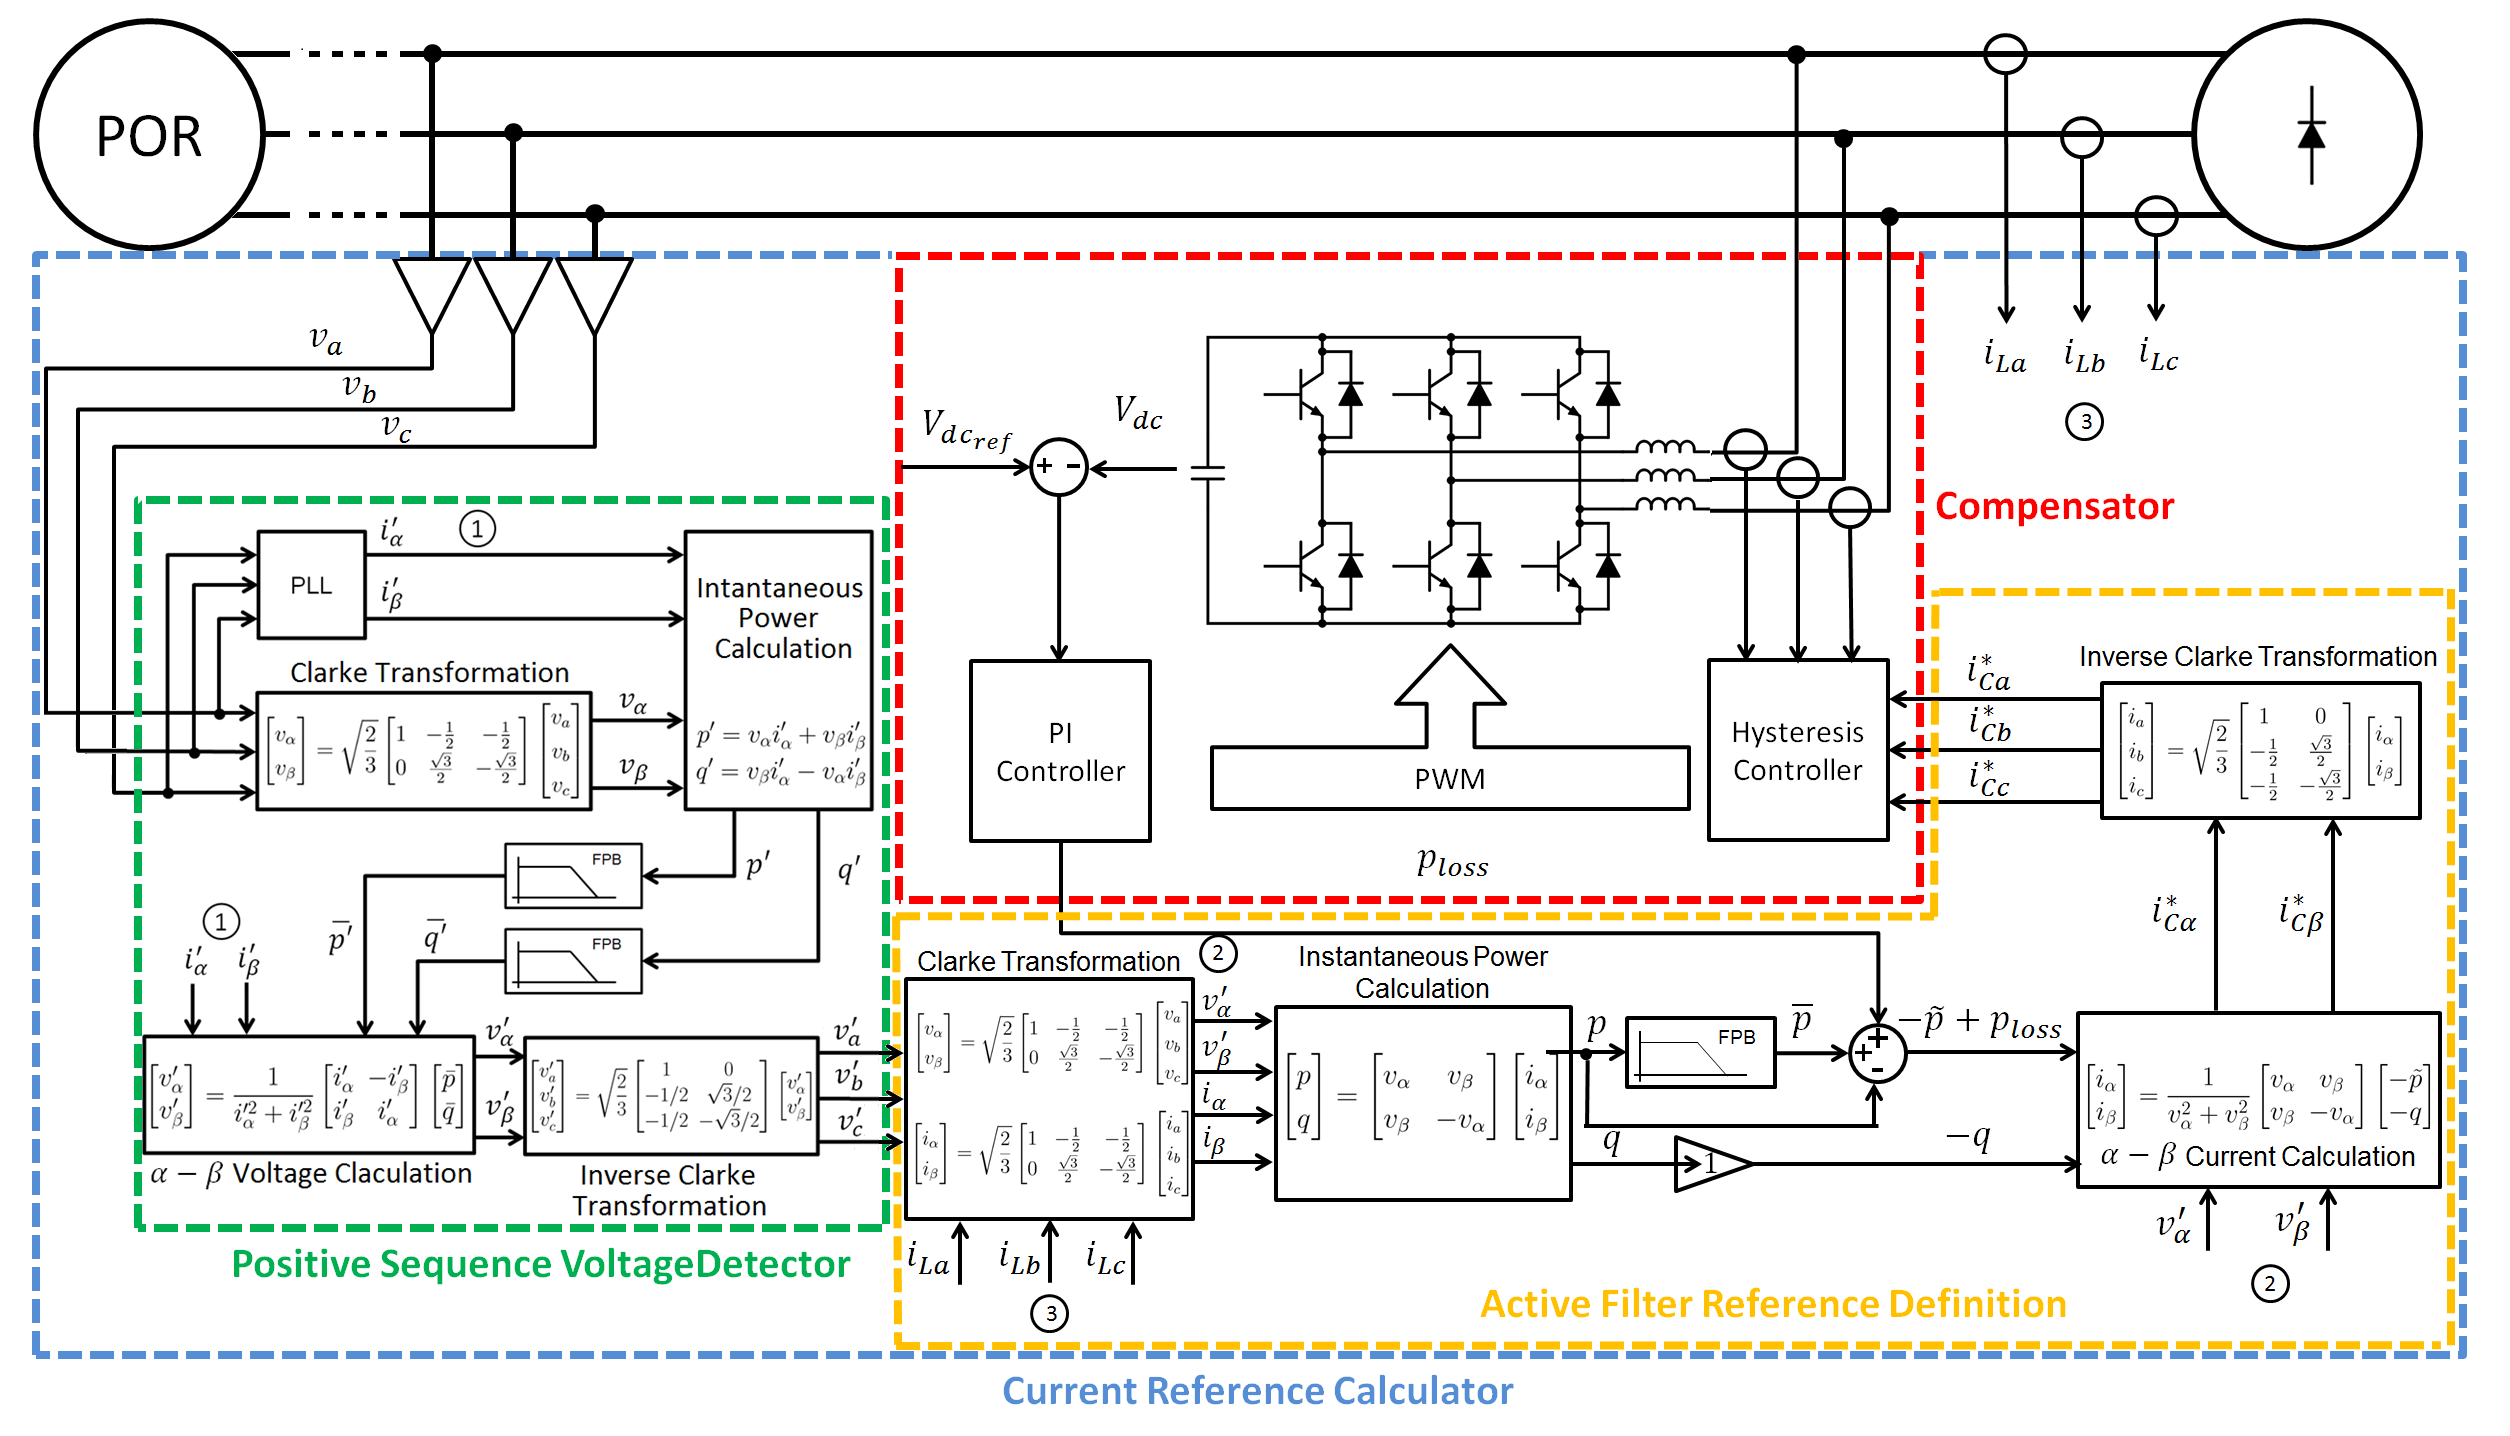
\includegraphics[width=0.99\textwidth]{Figures/filtro_blocos_1.png}
	\caption{Shunt active filter scheme}
	\label{fig:filtro_blocos_1.png}
\end{figure*}

\subsection{Electrical System Model}

The aircraft electrical system model considers the operation of the generation and distribution system with its respective non-idealities, which affect the power quality due to voltage drop. The simulation has a generator system, a power distribution system and three EHAs connected in parallel as the loads, see Fig. \ref{fig:simulacao_simulink.png}.

The generator system consists of a synchronous machine and a generator control unit (GCU). The GCU works as a field excitation controller to set the proper voltage in the POR. The synchronous machine also has resistance and inductive reactance connected in series with the voltage source to model the resistance and the inductance presented in the generator coils.

The power distribution system is composed of the transmission lines between the generator and the POR and between the POR and EHAs. Probes in the POR measure the system voltages levels to be sent as the reference input to the GCU. The power transmission lines are modeled as resistance and inductive reactance in series for each of the 3 phase lines.

The EHA is a non-linear load, since its input has a 3-phase diode bridge. The EHAs model has a 3 phase Graetz diode bridge with a controlled current source placed in its respective DC side. The controlled current source operation recreates the apparent power consumption of a real EHA. Thereby, this guarantees the simulation of the distorted current waveforms generated by the EHA in real operation.

\begin{figure*}[!tb] %
	\centering
	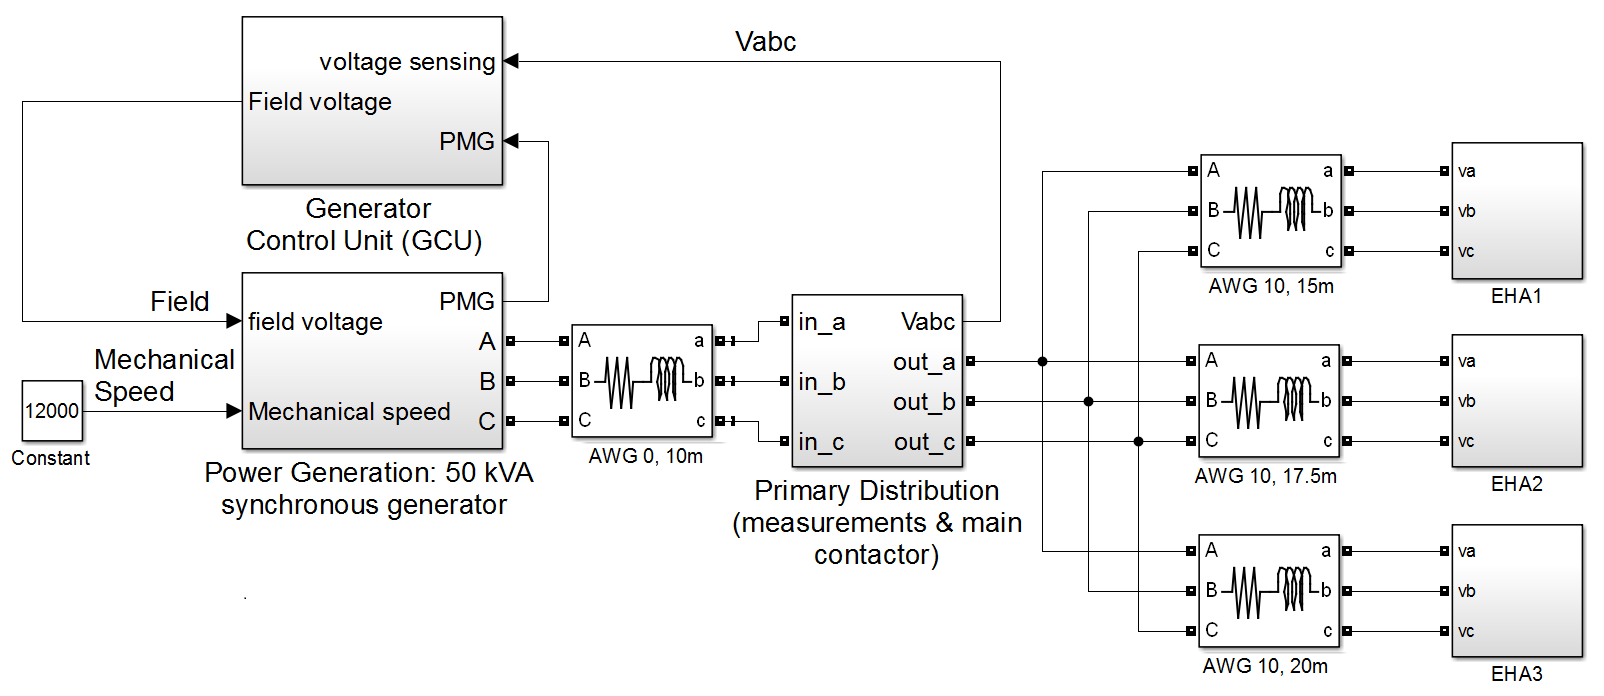
\includegraphics[width=0.9\textwidth]{Figures/simulacao_simulink.png}
	\caption{Electrical generation and distribution model}
	\label{fig:simulacao_simulink.png}
\end{figure*}

\subsection{Results}

The simulation results show the voltages and currents waveforms measured in the POR, the voltage frequency spectrum, the amplitude constraints defined by the MIL-STD 704F, and the calculated value of the voltage THD.

The test is divided in two conditions: the EHAs without operating and the EHAs starting their operation (maximum load). The results also show the cases where the active filters are connected and disconnected from the EHAs power input.

Fig. \ref{fig:artigo_unfilt_1.eps} and Fig. \ref{fig:artigo_unfilt_2.eps} show the system waveforms without active filters in the EHAs power inputs, when the EHAs are not in operation. Fig. \ref{fig:artigo_filt_1.eps} and Fig. \ref{fig:artigo_filt_2.eps} show the waveforms with the active filters connected to the EHAs power input for the same period. The active filters degrade the power quality during this time interval, since the THD increases and the frequency spectrum presents more harmonic content. This noise inserted in the system is due to the commutation of the VSC switching devices. Thus, even with the presence of the capacitor filter in the lines, some high frequency content injected in the grid was observed. However, the results are inside the limits defined by aeronautical standards.

Fig. \ref{fig:artigo_unfilt_3.eps} and Fig. \ref{fig:artigo_unfilt_4.eps} show the system waveforms without active filters connected to the grid, with the EHAs requiring maximum current. In the same time interval, Fig. \ref{fig:artigo_filt_3.eps} and Fig. \ref{fig:artigo_filt_4.eps} show the waveforms with the active filters connected to the EHAs power input. During this interval, it is clear the active filter enhancement in the system power quality. Considering these results, the active filter mitigates the harmonic content and set it within the limits of the MIL-STD 704F.

\begin{doublespacing}
	
	
	
	\begin{figure*}[!htb] %Circuito típico de um retificador de 12 pulsos com sua respectiva corrente de entrada
		\centering
		\begin{subfigure}[b]{0.5\textwidth}
			\centering
			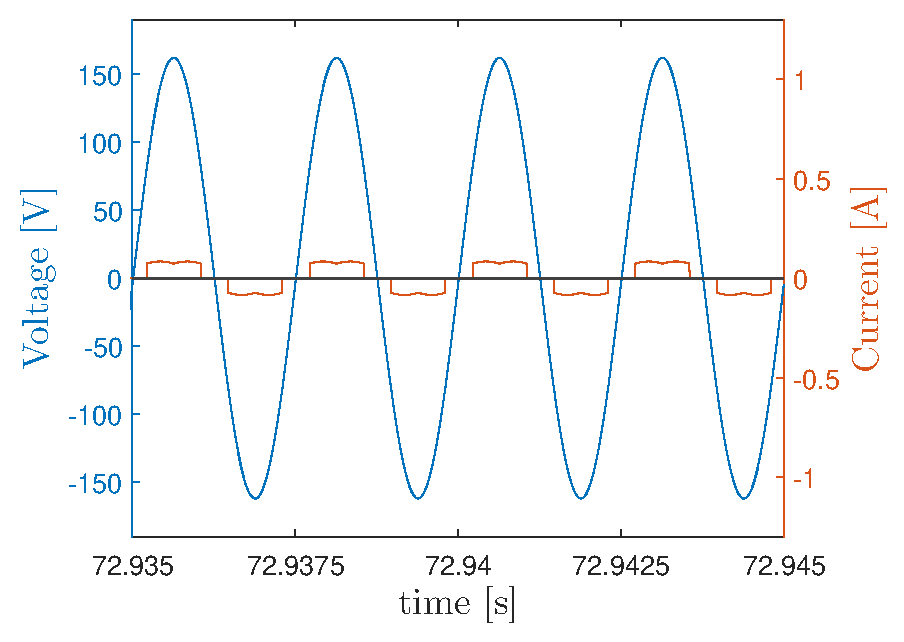
\includegraphics[height=5.5cm]{Figures/artigo_unfilt_1.eps}
			\caption{Voltage and current waveforms} 
			\label{fig:artigo_unfilt_1.eps}
		\end{subfigure}%
		\hfill
		\begin{subfigure}[b]{0.5\textwidth}  
			\centering 
			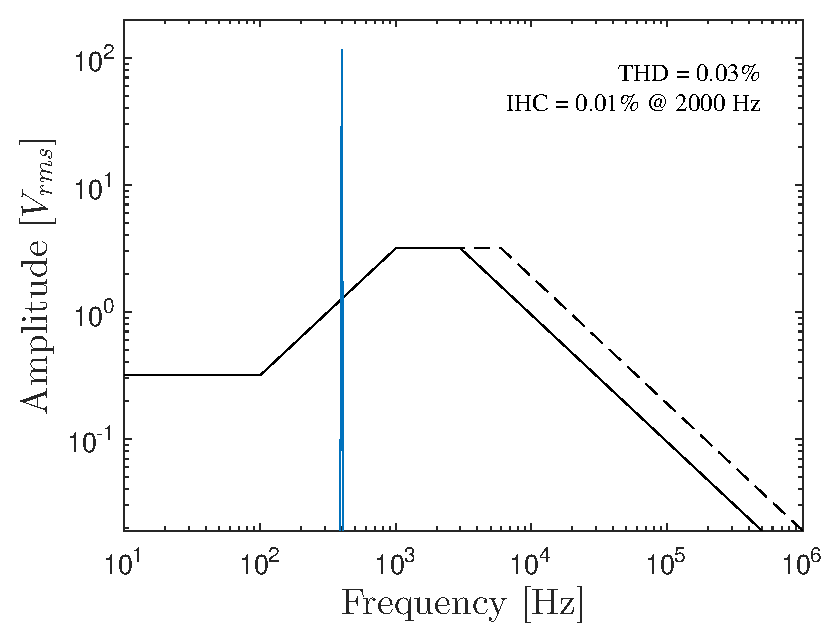
\includegraphics[height=5.5cm]{Figures/artigo_unfilt_2.eps}
			\caption{Voltage spectrum}    
			\label{fig:artigo_unfilt_2.eps}
		\end{subfigure}%
		\caption{System without load and filter}
		\label{fig:1}
	\end{figure*}
	
	\begin{figure*}[!htb] %Circuito típico de um retificador de 12 pulsos com sua respectiva corrente de entrada
		\centering
		\begin{subfigure}[b]{0.5\textwidth}
			\centering
			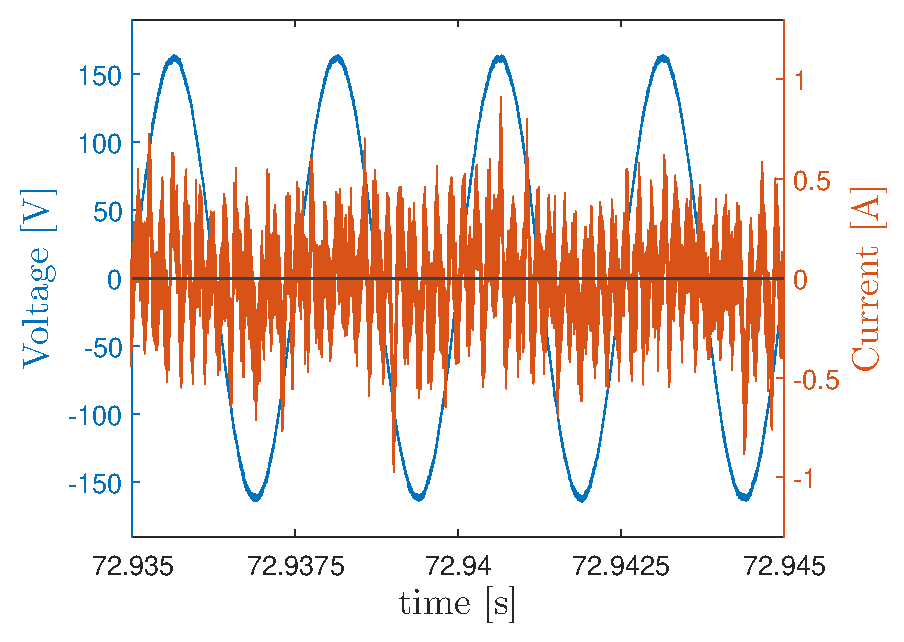
\includegraphics[height=5.5cm]{Figures/artigo_filt_1.eps}
			\caption{Voltage and current waveforms} 
			\label{fig:artigo_filt_1.eps}
		\end{subfigure}%
		\hfill
		\begin{subfigure}[b]{0.5\textwidth}  
			\centering 
			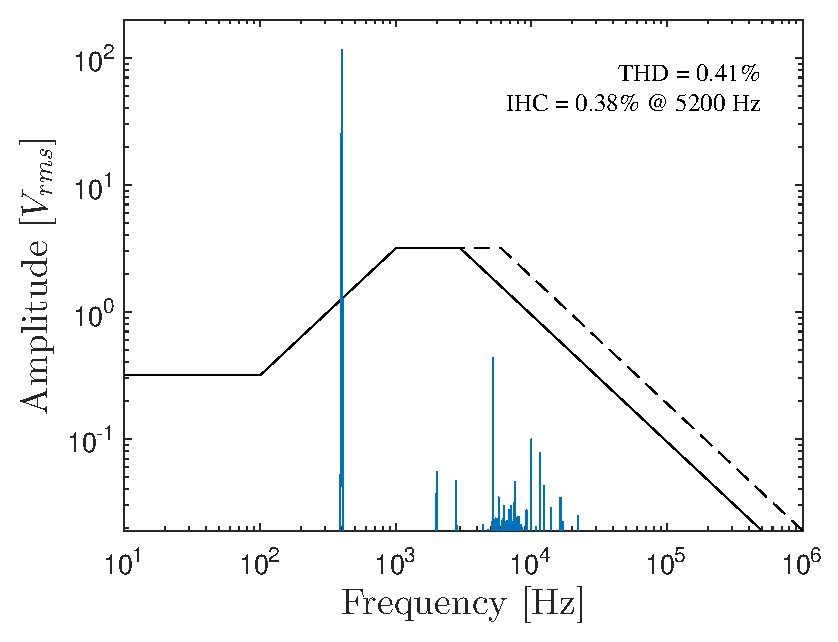
\includegraphics[height=5.5cm]{Figures/artigo_filt_2.eps}
			\caption{Voltage spectrum}    
			\label{fig:artigo_filt_2.eps}
		\end{subfigure}%
		\caption{System without load and with filter}
		\label{fig:2}
	\end{figure*}
	
	\begin{figure*}[!htb] %Circuito típico de um retificador de 12 pulsos com sua respectiva corrente de entrada
		\centering
		\begin{subfigure}[b]{0.5\textwidth}
			\centering
			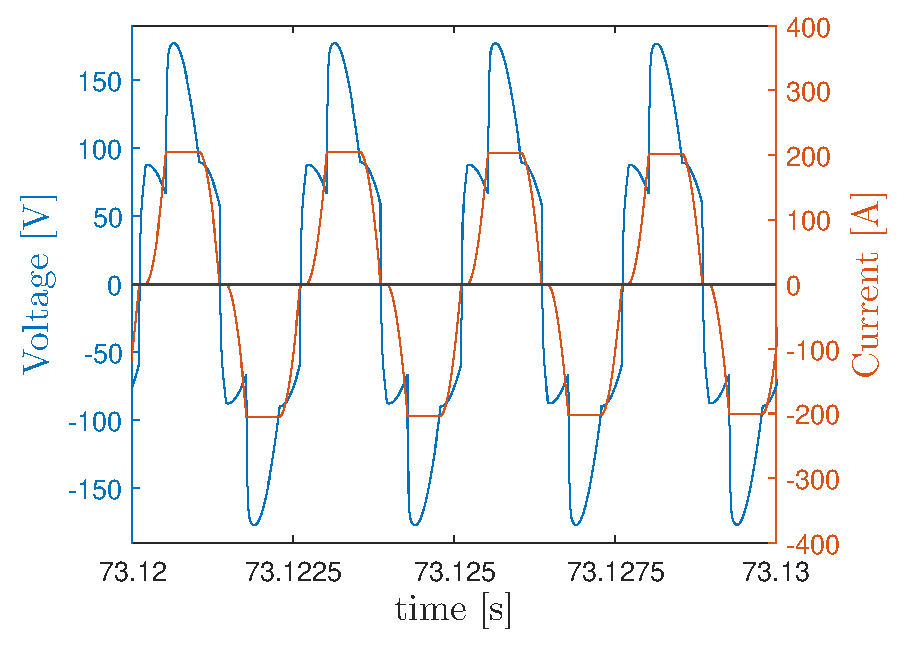
\includegraphics[height=5.5cm]{Figures/artigo_unfilt_3.eps}
			\caption{Voltage and current waveforms} 
			\label{fig:artigo_unfilt_3.eps}
		\end{subfigure}%
		\hfill
		\begin{subfigure}[b]{0.5\textwidth}  
			\centering 
			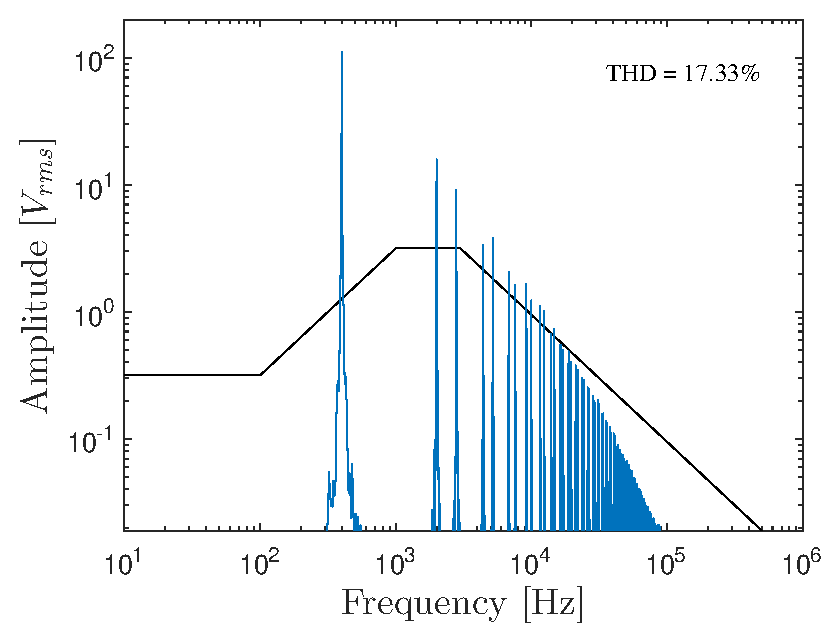
\includegraphics[height=5.5cm]{Figures/artigo_unfilt_4.eps}
			\caption{Voltage spectrum}    
			\label{fig:artigo_unfilt_4.eps}
		\end{subfigure}%
		\caption{System with load and without filter}
		\label{fig:3}
	\end{figure*}
	
	\begin{figure*}[!htb] %Circuito típico de um retificador de 12 pulsos com sua respectiva corrente de entrada
		\centering
		\begin{subfigure}[b]{0.5\textwidth}
			\centering
			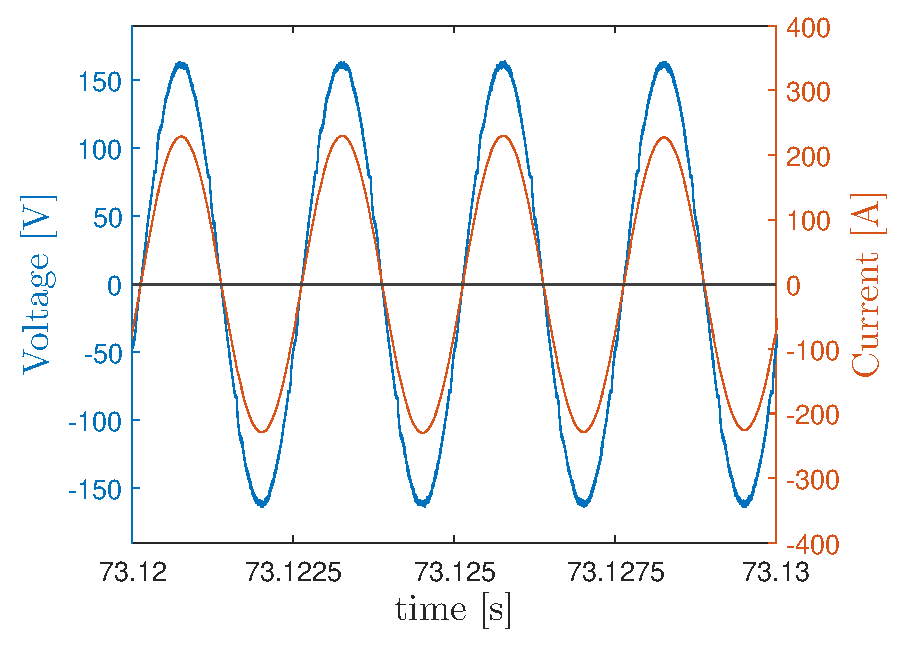
\includegraphics[height=5.5cm]{Figures/artigo_filt_3.eps}
			\caption{Voltage and current waveforms} 
			\label{fig:artigo_filt_3.eps}
		\end{subfigure}%
		\hfill
		\begin{subfigure}[b]{0.5\textwidth}  
			\centering 
			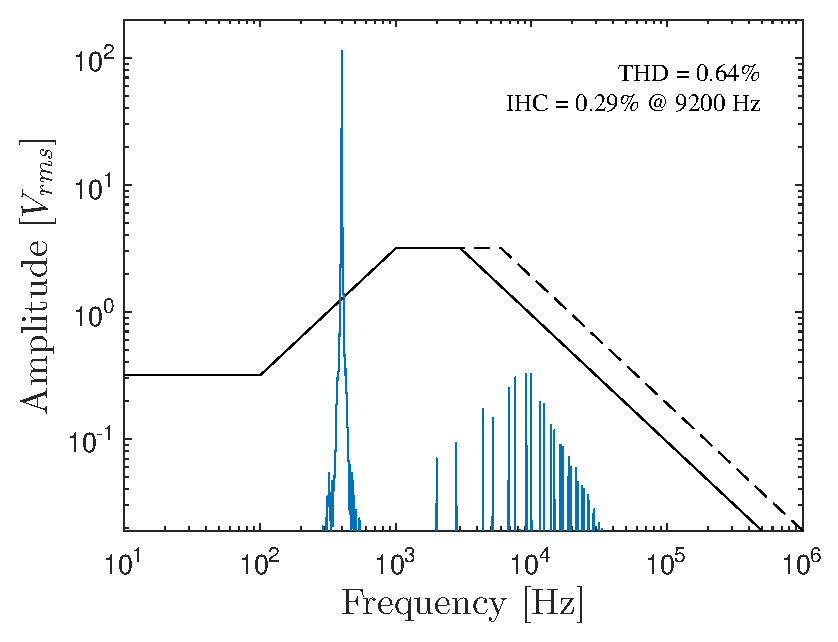
\includegraphics[height=5.5cm]{Figures/artigo_filt_4.eps}
			\caption{Voltage spectrum}    
			\label{fig:artigo_filt_4.eps}
		\end{subfigure}%
		\caption{System with load and filter}
		\label{fig:4}
	\end{figure*}
	
\end{doublespacing}
\FloatBarrier